\documentclass[10pt,conference,compsocconf]{IEEEtran}

\usepackage{hyperref}
\usepackage{graphicx}	% For figure environment


\begin{document}
\title{Machine Learning -- Project 1}

\author{
  Pierre Fouche, Matthias Leroy and Alexandre Poussard\\
  \textit{MSc Data Science -- EPFL, Switzerland}
}

\maketitle

\begin{abstract}
  The aim of this paper is to make classification of particles over results' experiments. Thus, given a set of features that describe the decay signature of a collision event, we tried to predict if this event was a Higgs boson signal or some background information. We will expose the different machine learning algorithms we tried and the evaluations we made that finally led us to the ridge regression.
\end{abstract}

\section{Features Analysis and Data Preparation}

The training set is composed of 250 000 samples of each 30 features representing 30 experimental measurements. During our dataset exploratory analysis, we noticed that the 23rd feature (\textit{PRI.jet.num}) is discrete and categorical with values in the set $\{0,1,2,3\}$ whereas all the other features were continuous. Moreover, the documentation of the contest (LIEN LIEN) explained the dependence between the 23rd column and all the other ones (some ones are not defined ($-999$) according to the value of \textit{PRI.jet.num}. That is why, we though it was a good idea to divide our data in three different sets according to the \textit{PRI.jet.num} values (2 and 3 have the same features dependence, that's why we combined these sets). Thus, we could drop uninteresting features for each sets, that could allowed us to optimize the training. However, despite this first cleaning, we realise that we still had non-defined values ($-999$) in the first feature (\textit{DER.mass.MMC}). Thus, we decided to split again our three sets in 2 smaller ones which containes defined or non-defined values in \textit{DER.mass.MMC} feature (and we drop this column for the non-defined ones).
Finally, we had six datasets depending on textit{PRI.jet.num} and \textit{DER.mass.MMC} with only defined values. This allows us to have two benefits for the computations: smaller training dataset and more precise one.

%We then decided to divide our training set into 3 subsets (because number 2 and 3 have the same -999). Then in the doc, they explained depending on those 4 categories, other features are defined or not which allows us to split the data based on these categrôries. We also notice that for 2 and 3, features are defined in the same way and so we can merge data set 2/3 and obtain 3 datasets. 
%However, we still have non-defined values in the first column (DER.mass.MMC) and we decide to split again for each Jet into 2 smaller datasets which containes defined OR nondefined values.
%We then have 6 datasets depending on jets and Mass and with only defined values. This allows us to have two benefits: smaller training dataset (for computation) and more precise one. \\

Then, we standardized each dataset and focus on polynomial basis. Thus, for each subset, we have at the beginning N rows and D features. For the polynomial basis, which goal is to add other features for better training, we then have a subset with still N rows but D*d (d = max degree). This degree is defined thanks to the cross-validation according to the model we use. See Section~\ref{sec:Models and Methods}. Instead of trying to find a different degree for each training dataset we could have chosen a common one big enough to satisfied each set. We would gain in test rapidity but risk to overfit the data. Then, we decide to add more features by modifying and combining existing ones depending on our training set. In fact, features engineering increase considerably our classification precision, but in return our training model asked for more memory and take longer to process. Thus, we try different method in order to find the best trad-off that we could make for each training set. First of all we compute the cross term matrix of our D original features (the one to one product for each column) and get C = (D*(D-1))/2 new features. Then, we decide to add the square, square root and cubic root of these combinations. Thus, if we apply each of these new features of one of our training set, it will be finally composed of N samples and D*d+C*4 features. However, we did not add all these features to all of our training set. In fact, we evaluate the importance of each one of them with our cross validation test and populate our set according to the losses we get. 

%and features engineering. However, this is more detailed in the last part of this report since we first implemented our models and then we tried to improve them, and paricularly with features processing\\

\section{Models and Methods}
\label{sec:structure-paper}

In order to make our predictions, we tested 6 different machine learning methods, that we tried to improve according to the results, and the validation evaluations we got. Thus, we started to think about the better way to evaluate our models, and we finnaly decided to implement a 5-fold cross-validation (it seems to us a raisonnable choice since we got validation sets of 50 000 samples which is equivalent to a $20\%-80\%$ split of test and training data). 

First of all, we tried a linear regression using a gradient descent. Our first questioning was to find a correct learning rate $\gamma$ in order to converge to the best parameters $\mathbf{w^*}$ for the minimum cost function that we could possibly find with this optimization algorithm. After testing different values for $\gamma$ it was finally possible to make our first prediction. It was very encouraging but we want to test other algorithm before started to optimize one. Thus, we implemented a stochastic gradient descent. We had to use a standard mini-batch-size-1. We did the same work, and try to optimize the step-size. However, whatever its value was, we did not succed to find a smaller loss that we got with the batch gradient descent. The only benefit of this methods was the computational cost, in fact the convergence's speed was a little bit faster. However, at this step of the challenge, we were more concerned about efficency and  precision of the results rather than complexity as long as our computer succeeded to get a result. Morever, we could have tried mini-batch SGD and found a trade-off between speed and loss. However, we could most probably not have a better loss than with gradient descent and we did not want to persevere knowing that we could find optimum $\mathbf{w^*}$ parameters with least squares regression using normal equations. Actually, the solution is obtained explicitly by solving these normal equations and thus, optimize what we tried to do with gradient descents models. We get indeed better predictions using Least Square and we get a categorization accuracy of (----) on Kaggle. From this result, we tried to improve it with extended features vectors. Thus, we added a polynomial basis in order to increase the representiational power of the linear model. That's why we ran our cross-validation in order to determine the degree M that minimize our validation error for each of our 6 training sets. And we finally got our best prediction score. However, we noticed that the error for the training sets and the validation sets occasionally disgressed a little for the best degrees. Thus, it could be resulting of an overfiting problem. Therefore, in order to reduce our variance we tried to regularize our linear model by using ridge regression using normal equations. In fact, most of the work was to determine the hyperparameters, since for this model we have to find a $\lambda$ parameter that best regularize our model by penalize complex ones for every polynomial basis we wanted to test. Therefore, after runing our 5-fold cross-validation w find a set of 6 $degre, \lambda$ couples for each dataset, that minimize the losses. Finally, we got a better prevision than with the Least Square model, we obtained (----) on Kaggle. Surprisingly, the $lambdas$ that gave us the best results were a bit small, thus, Least Square model was not overfitting that much.
Then, we implemented the logistic regression with gradient descent. We had good hope for this model because it is supposed to be optimized for classification problems. However, after training our data and find 
our learning rate  hyperparameter $\gamma$ (for the gradient descent) and the degrees of our polynomial basis. We were not able to reduce the loss compared to the ridge regression. In fact, we got a prediction score of (-----) on kaggle, which was close but not good enough.
Finally, we did not succed to implement the regularized logistic regression. Our cross validation never converge and we were not able to find our best hyperparameters for this models.

%the \textit{Newton's method} that we tried did not satisfy us. Indeed, we had hard time to compute our parameters $\gamma$ (for the gradient descent) and the degrees of our polynomial basis. In fact, the \textit{Hessian} of the loss function was very costly, and we did not succeed to estimate a good estimation (it seems that our computers had not enough memory for the work we asked). And finally, our results was worst than for the  ridge regression. Then, we implement a regularized logistic regression...

\section{Improving Prediction}

After, we found our best prediction, we asked ourself how we could continue to improve it. In fact, at the begining of the challenge we tried models we have implemented directly on the 30 features dataset we downloaded. Without thinking about features engineering. It ended up with a very high bias over our estimation. In fact, it was not bother us to much when we start because the training and validation errors were very close when we ran the cross validation but, the error itself was not small enough for our prediction goal. That is why, \\
\\
\\

Scientific papers usually begin with the description of the problem,
justifying why the problem is interesting. Most importantly, it argues
that the problem is still unsolved, or that the current solutions are
unsatisfactory. This leads to the main gist of the paper, which is
``the idea''. The authors then show evidence, using derivations or
experiments, that the idea works. Since science does not occur in a
vacuum, a proper comparison to the current state of the art is often
part of the results. Following these ideas, papers usually have the
following structure:
\begin{description}
\item[Abstract] \ \\
  Short description of the whole paper, to help the
  reader decide whether to read it.
\item[Introduction] \ \\
  Describe your problem and state your
  contributions.
\item[Models and Methods] \ \\
  Describe your idea and how it was implemented to solve
  the problem. Survey the related work, giving credit where credit is
  due.
\item[Results] \ \\
  Show evidence to support your claims made in the
  introduction.
\item[Discussion] \ \\
  Discuss the strengths and weaknesses of your
  approach, based on the results. Point out the implications of your
  novel idea on the application concerned.
\item[Summary] \ \\
  Summarize your contributions in light of the new
  results.
\end{description}


\section{Tips for Good Writing}
\label{sec:tips-writing}

The ideas for good writing have come
from~\cite{editor10,jones08,anderson04}.

\subsection{Getting Help}
One should try to get a draft read by as many friendly people as
possible. And remember to treat your test readers with respect. If
they are unable to understand something in your paper, then it is
highly likely that your reviewers will not understand it
either. Therefore, do not be defensive about the criticisms you get,
but use it as an opportunity to improve the paper. Before your submit
your friends to the pain of reading your draft, please \emph{use a
  spell checker}.

\subsection{Abstract}
The abstract should really be written last, along with the title of
the paper. The four points that should be covered~\cite{jones08}:
\begin{enumerate}
\item State the problem.
\item Say why it is an interesting problem.
\item Say what your solution achieves.
\item Say what follows from your solution.
\end{enumerate}

\subsection{Figures and Tables}

\begin{figure}[tbp]
  \centering
  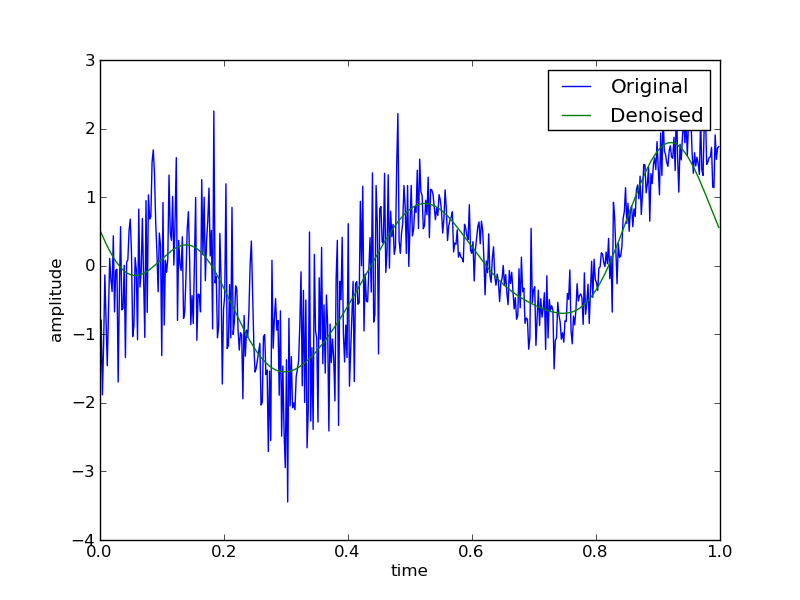
\includegraphics[width=\columnwidth]{denoised_signal_1d}
  \caption{Signal compression and denoising using the Fourier basis.}
  \vspace{-3mm}
  \label{fig:denoise-fourier}
\end{figure}
\begin{figure}[htbp]
  \centering
  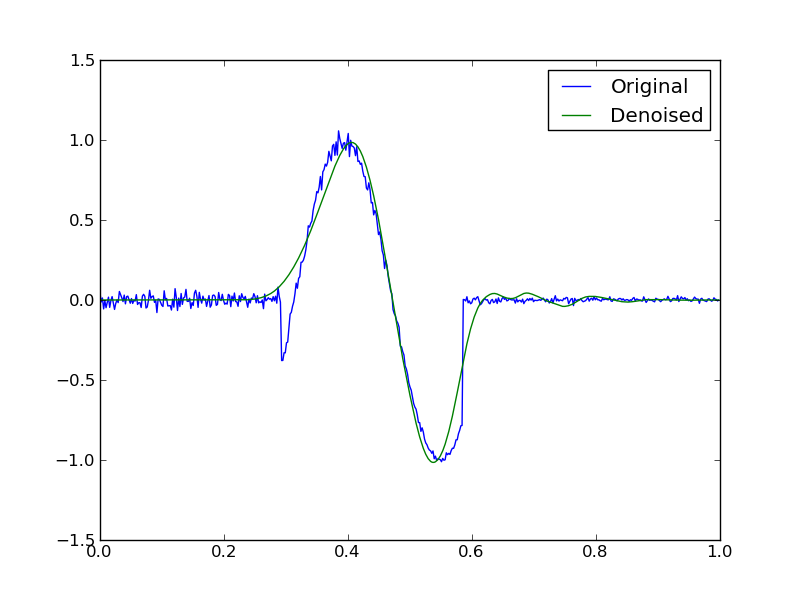
\includegraphics[width=\columnwidth]{local_wdenoised_1d}
  \vspace{-3mm}
  \caption{Signal compression and denoising using the Daubechies wavelet basis.}
  \label{fig:denoise-wavelet}
\end{figure}

Use examples and illustrations to clarify ideas and results. For
example, by comparing Figure~\ref{fig:denoise-fourier} and
Figure~\ref{fig:denoise-wavelet}, we can see the two different
situations where Fourier and wavelet basis perform well. 

\subsection{Models and Methods}
The models and methods
section should describe what was
done to answer the research question, describe how it was done,
justify the experimental design, and
explain how the results were analyzed.

The model refers to the underlying mathematical model or structure which 
you use to describe your problem, or that your solution is based on. 
The methods on the other hand, are the algorithms used to solve the problem. 
In some cases, the suggested method directly solves the problem, without having it 
stated in terms of an underlying model. Generally though it is a better practice to have 
the model figured out and stated clearly, rather than presenting a method without specifying 
the model. In this case, the method can be more easily evaluated in the task of fitting 
the given data to the underlying model.

The methods part of this section, is not a step-by-step, directive,
protocol as you might see in your lab manual, but detailed enough such
that an interested reader can reproduce your
work~\cite{anderson04,wavelab}.

The methods section of a research paper provides the information by
which a study's validity is judged.
Therefore, it requires a clear and precise description of how an
experiment was done, and the rationale
for why specific experimental procedures were chosen.
It is usually helpful to
structure the methods section by~\cite{kallet04methods}:
\begin{enumerate}
\item Layout the model you used to describe the problem or the solution.
\item Describing the algorithms used in the study, briefly including
  details such as hyperparameter values (e.g. thresholds), and
  preprocessing steps (e.g. normalizing the data to have mean value of
  zero).
\item Explaining how the materials were prepared, for example the
  images used and their resolution.
\item Describing the research protocol, for example which examples
  were used for estimating the parameters (training) and which were
  used for computing performance.
\item Explaining how measurements were made and what
  calculations were performed. Do not reproduce the full source code in
  the paper, but explain the key steps.
\end{enumerate}

\subsection{Results}

Organize the results section based on the sequence of table and
figures you include. Prepare the tables and figures as soon as all
the data are analyzed and arrange them in the sequence that best
presents your findings in a logical way. A good strategy is to note,
on a draft of each table or figure, the one or two key results you
want to address in the text portion of the results.
The information from the figures is
summarized in Table~\ref{tab:fourier-wavelet}.

\begin{table*}[htbp]
  \centering
  \begin{tabular}[c]{|l||l|l|l|}
    \hline
    Basis&Support&Suitable signals&Unsuitable signals\\
    \hline
    Fourier&global&sine like&localized\\
    wavelet&local&localized&sine like\\
    \hline
  \end{tabular}
  \caption{Characteristics of Fourier and wavelet basis.}
  \label{tab:fourier-wavelet}
\end{table*}

When reporting computational or measurement results, always
report the mean (average value) along with a measure of variability
(standard deviation(s) or standard error of the mean).


\section{Tips for Good Software}
\label{sec:tips-software}

There is a lot of literature (for example~\cite{hunt99pragmatic} and
\cite{spolsky04software}) on how to write software. It is not the
intention of this section to replace software engineering
courses. However, in the interests of reproducible
research~\cite{schwab00}, there are a few guidelines to make your
reader happy:
\begin{itemize}
\item Have a \texttt{README} file that (at least) describes what your
  software does, and which commands to run to obtain results. Also
  mention anything special that needs to be set up, such as
  toolboxes\footnote{For those who are
  particularly interested, other common structures can be found at
  \url{http://en.wikipedia.org/wiki/README} and
  \url{http://www.gnu.org/software/womb/gnits/}.}.
\item A list of authors and contributors can be included in a file
  called \texttt{AUTHORS}, acknowledging any help that you may have
  obtained. For small projects, this information is often also
  included in the \texttt{README}.
\item Use meaningful filenames, and not \texttt{temp1.py},
  \texttt{temp2.py}. 
\item Document your code. Each file should at least have a short
  description about its reason for existence. Non obvious steps in the
  code should be commented. Functions arguments and return values should be described.
\item Describe how the results presented in your paper can be reproduced.
\end{itemize}


\subsection{\LaTeX{} Primer}
\label{sec:latex-primer}

\LaTeX{} is one of the most commonly used document preparation systems
for scientific journals and conferences. It is based on the idea
that authors should be able to focus on the content of what they are
writing without being distracted by its visual presentation.
The source of this file can be used as a starting point for how to use
the different commands in \LaTeX{}. We are using an IEEE style for
this course.

\subsubsection{Installation}

There are various different packages available for processing \LaTeX{}
documents.
On OSX use Mac\TeX{}
(\url{http://www.tug.org/mactex/}). On Windows, use for example Mik\TeX{} (\url{http://miktex.org/}).

\subsubsection{Compiling \LaTeX{}}
Your directory should contain at least~4 files, in addition to image
files. Images should be in \texttt{.png}, \texttt{.jpg} or
\texttt{.pdf} format.
\begin{itemize}
\item IEEEtran.cls
\item IEEEtran.bst
\item groupXX-submission.tex
\item groupXX-literature.bib
\end{itemize}
Note that you should replace groupXX with your chosen group name.
Then, from the command line, type:
\begin{verbatim}
$ pdflatex groupXX-submission
$ bibtex groupXX-literature
$ pdflatex groupXX-submission
$ pdflatex groupXX-submission
\end{verbatim}
This should give you a PDF document \texttt{groupXX-submission.pdf}.

\subsubsection{Equations}

There are three types of equations available: inline equations, for
example $y=mx + c$, which appear in the text, unnumbered equations
$$y=mx + c,$$
which are presented on a line on its own, and numbered equations
\begin{equation}
  \label{eq:linear}
  y = mx + c
\end{equation}
which you can refer to at a later point (Equation~(\ref{eq:linear})).

\subsubsection{Tables and Figures}

Tables and figures are ``floating'' objects, which means that the text
can flow around it.
Note
that \texttt{figure*} and \texttt{table*} cause the corresponding
figure or table to span both columns.



\section{Summary}

The aim of a scientific paper is to convey the idea or discovery of
the researcher to the minds of the readers. The associated software
package provides the relevant details, which are often only briefly
explained in the paper, such that the research can be reproduced.
To write good papers, identify your key idea, make your contributions
explicit, and use examples and illustrations to describe the problems
and solutions.

\section*{Acknowledgements}
The author thanks Christian Sigg for his careful reading and helpful
suggestions.

\bibliographystyle{IEEEtran}
\bibliography{literature}

\end{document}
